\documentclass[12pt]{article}
\title{Dokumentacja implementacji algorytmu wstecznej propagacji na przykładzie funkcji NXoR}
\author{Michał Korniak}
\date{}
\usepackage{graphicx}
\usepackage{graphics}
\usepackage[polish]{babel}
\usepackage[T1]{fontenc}
\newcommand{\source}[1]{{\centerline{\tiny Źródło: #1}}}

\usepackage{color}
\definecolor{bluekeywords}{rgb}{0.13,0.13,1}
\definecolor{greencomments}{rgb}{0,0.5,0}
\definecolor{redstrings}{rgb}{0.9,0,0}

\usepackage{listings}
\lstset{language=[Sharp]C,
  showspaces=false,
  showtabs=false,
  breaklines=true,
  showstringspaces=false,
  breakatwhitespace=true,
  escapeinside={(*@}{@*)},
  commentstyle=\color{greencomments},
  keywordstyle=\color{bluekeywords},
  stringstyle=\color{redstrings},
  basicstyle=\footnotesize,
  numbers=left,
  xleftmargin=5.0ex,
}
 


\begin{document}
\maketitle
\tableofcontents{}
\newpage


\section{Wprowadzenie}
Algorytm wstecznej propagacji błędu jest metodą uczenia wielowarstwowych polegającą na korekcie wag połączeń między neuronami na podstawie błędu całej sieci.
W tym dokumencie prześledzę działanie tego algorytmu na przykładzie sieci realizującej funkcję NXoR,
jednocześnie przedstawiając jego autorską implementację w języku C\#.

\section{Algorytm wstecznej propagacji}
\subsection{Sposób działania wielowarstwowych sieci neuronowych}
Algorytm wstecznej propagacji jest wykorzystywany do nauczania wielowarstwowych sieci jednokierunkowych.
Taka sieć zawiera warstwę wejściową i warstwę wyjściową,
może posiadać również warstwy ukryte (w zależności od problemu jedną albo dwie).
Każda warstwa zawiera dowolną ilość neuronów.
Neurony są połączone ze sobą w taki sposób, że każdy neuron warstwy innej niż wyjściowa jest połączony z każdym neuronem kolejnej warstwy,
a każde połączenie ma określoną wagę.
Dodatkowo możliwe jest połączenie do tego zwanego biasa, czyli połączenia do neuronu, który zawsze przyjmuje wartość 1.
Połączenia wejściowe do neuronu będą wpływać na to jaką będzie miał wartość.

Rysunek 1 przedstawia przykład jednokierunkowej sieci neuronowej opartej o dwa neurony warstwy wejściowej i tyle samo neuronów w warstwach ukrytej i wyjściowej. 
Oprócz połączeń do innych neuronów, istnieją również połączenia do biasa, który jest wspólny dla neuronów w ramach jednej warstwy.

\begin{figure}[!ht]
    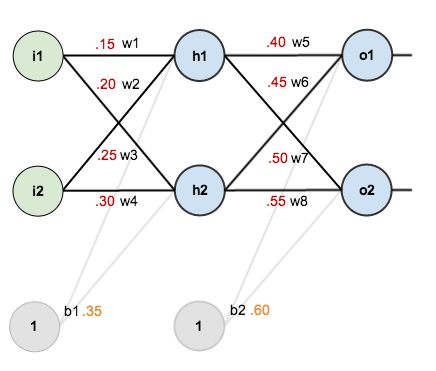
\includegraphics[width=\linewidth]{images/feed-forward-diagram.png}
    \source{https://mattmazur.com/2015/03/17/a-step-by-step-backpropagation-example/}
    \caption{Przykład wielowarstwowej sieci jednokierunkowej}
\end{figure}

Rysunek 1 zawiera wartości neuronów wejściowych oraz wag, dzięki czemu będziemy mogli pokazać jak wyliczane są wartości kolejnych neuronów.
Robimy to sumując wartości połączeń do tego wektora, a następnie poddając wynik funkcji aktywacji.
Przez wartość połączenia będziemy rozumieli iloczyn wagi i neuronu wejściowego dla połączenia.
Przykładowo dla neuronu h1 wartość przed użyciem funkcji aktywacji będzie równa:
\[
  net = i1*w1+i2*w2+1*b1
\]
Co po podstawieniu wartości da:
\[
  net_{h1} = 0.05*0.15+0.10*0.20+1*0.35=0.3775
\]
Taka wartość jest następnie poddawana działaniu funkcji aktywacji. 
Takie działanie umożliwia normalizowanie wartości neuronów do oczekiwanych przedziałów wartości.
W tym przypadku skorzystamy z funkcji sigmoidalnej, której zakres wartości mieści się w przedziale [0,1]:
\[
    f(x) =  \frac{\mathrm{1} }{\mathrm{1} + e^{-x} } 
\]
Po podstawieniu otrzymanej wcześniej wartości do funkcji dostaniemy wartość neuronu h1:
\[
    out_{h1} 
    = f(net_{h1}) 
    =  \frac{\mathrm{1} }{\mathrm{1} + e^{-net_{h1}} } 
    =  \frac{\mathrm{1} }{\mathrm{1} + e^{-0.3775} } \approx 0.5932
\]
W ten sposób będziemy liczyć wartość kolejnych neuronów aż otrzymamy wynik.

\subsection{Implementacja wielowarstwowej sieci neuronowej}

Teraz przedstawię implementację mechanizmu zaprezentowanego w poprzednim podrozdziale.
Jej podstawą jest klasa odwzorowującej sieć neuronową, w naszym przypadku
taką funkcję pełni klasa NeuralNetwork, która to implementuje interfejs pokazany na listingu \ref{lst:INeuralNetwork}.

\begin{lstlisting}[caption={Interfejs INeuralNetwork}, label={lst:INeuralNetwork}]
  public interface INeuralNetwork
  {
      IEnumerable<IInputNeuron> InputLayer { get; }
      IEnumerable<IHiddenNeuron> HiddenLayer { get; }
      IEnumerable<IOutputNeuron> OutputLayer { get; }
      IErrorFunction ErrorFunction { get; }
      void FillInputNeurons(IEnumerable<double> input);
      IEnumerable<double> CalculateOutput();
  }
\end{lstlisting}

W tym momencie skupmy się na linijkach 3, 4 i 5, które to wskazują na to, że sieć neuronowa zawiera warstwy wejściową, ukrytą i wyjściową.
Jak widzimy każda warstwa posiada inny typ neuronu, co wynika to z tego, że w zależności od warstwy neurony się różnią. Przykładowo:
\begin{itemize}
  \item Neuron warstwy wejściowej nie ma możliwości dodawanie połączeń wejściowych.
  \item Neuron warstwy wyjściowej nie ma możliwości dodawanie połączeń wyjściowych.
  \item Neuron warstwy ukrytej ma możliwość dodawanie obu typów połączeń.
\end{itemize}

Obiekt klasy NeuralNetwork jest tworzony z wykorzystaniem wzorca "Builder".
Dzieje się to w sposób pokazany na listingu \ref{lst:NeuralNetworkBuilder}.

\begin{lstlisting} [caption={Budowanie obiektu NeuralNetwork},label={lst:NeuralNetworkBuilder}]
  var neuralNetworkBuilder = new NeuralNetworkBuilder();
  var network = neuralNetworkBuilder
      .SetNumberOfInputNeurons(2)
      .SetNumberOfOutputNeurons(1)
      .SetActivationFunction(new SigmoidActivationFunction())
      .SetErrorFunction(new MeanSquaredErrorFunction(1))
      .SetNumberOfHiddenNeurons(3)  //opcjonalne
      .AddBiasConnections()         //opcjonalne
      .Build();
\end{lstlisting}

Klasa NeuralNetworkBuilder umożliwia stworzenie sieci neuronowej:
\begin{itemize}
  \item Zawierającą wybraną ilość neuronów warstwy wejściowej.
  \item Zawierającą wybraną ilość neuronów warstwy wyjściowej
  \item Działającą na określonej funkcji aktywacji
  \item Wyliczającej błąd na podstawie wybranej funkcji
  \item Umożliwiającej opcjonalne dodanie warstwy ukrytej
  \item Umożliwiającej opcjonalne dodanie połączeń do biasów
\end{itemize}

Zadaniem Buildera jest stworzenie obiektu klasy NeuralNetwork, który spełni podane wymagania. 
W zależności od tego czy użytkownik będzie potrzebował warstwy ukrytej, Builder utworzy sieć która ma połączenia z warstwą pośrednią lub też bezpośrednie połączenia warstwy wejściowej z wyjściowej.
Podobnie jest z wyborem tego czy czy powinny być tworzone biasy czy też nie.
Builder nie posiada żadnej metody dotyczącej wyboru pierwotnych wag połączeń, wynika to z tego, że zgodnie z założeniem algorytmu wstecznej propagacji są one inicjalizowane losowo.

Dla tak stworzonej sieci neuronowej możemy przeprowadzić obliczenia, które zostały przedstawione w poprzednim podrozdziale.
Robimy to w sposób przedstawiony w listingu \ref{lst:CalculateOutput}

\begin{lstlisting} [caption={Budowanie obiektu NeuralNetwork},label={lst:CalculateOutput}]
  network.FillInputNeurons(new double[] { 0, 1 });
  var output = network.CalculateOutput();
\end{lstlisting}

W pierwszej kolejności są wypełniane neurony wejściowe.
Jeśli użytkownik poda liczbę danych wejściowych różniącą się od liczby neuronów warstwy wejściowej zostanie wyrzucony wyjątek.

Wyjście sieci jest liczone w sposób rekurencyjny:
\begin{itemize}
  \item Wyjście każdego neuronu z wyjątkiem neuronów wejściowych jest sumą wyjść połączeń wejściowych poddaną funkcji aktywacji (listing \ref{lst:NeuronOutput}).
  \item Wyjście połączenia jest iloczynem wagi i wyjścia neuronu źródłowego (listing \ref{lst:ConnectionOutput})
\end{itemize}

\begin{lstlisting} [caption={Budowanie obiektu NeuralNetwork},label={lst:NeuronOutput}]
  public class OutputNeuron : IOutputNeuron
  {
      //***
      public double NetOutput => _inputConnections.Sum(x => x.Output);
      public double Output => _activationFunction.Invoke(NetOutput);
      //***
  }
\end{lstlisting}


\begin{lstlisting} [caption={Budowanie obiektu NeuralNetwork},label={lst:ConnectionOutput}]
  class NeuronConnection: INeuronConnection
  {
      //***
      public double Output => Weight * _source.Output;
      //***
  }
\end{lstlisting}

\subsection{Trening sieci neuronowej}











\end{document}

